\begin{subsection}{Experimental Design and Modeling Objectives}

\begin{frame}{Experimental Design}

\begin{figure}
    	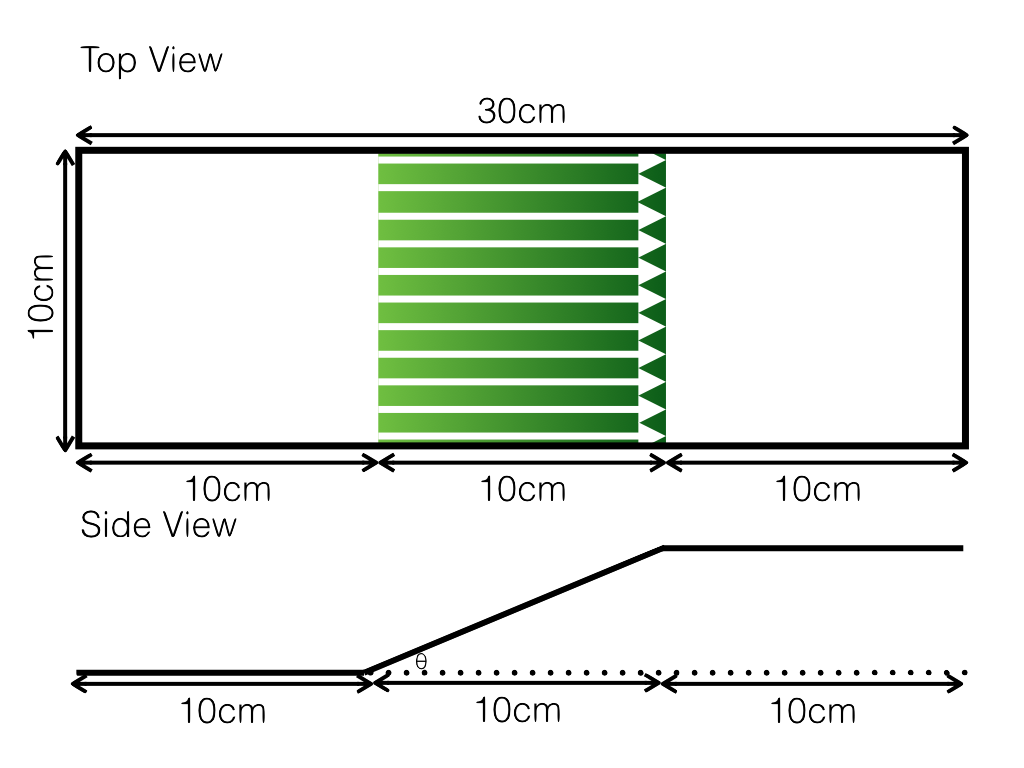
\includegraphics[width=0.8\textwidth]{images/model_components_cartoons_011}
      \caption{Arena terrain scheme}
 \end{figure}
\end{frame}

\begin{frame}{Modeling Objectives}
\vspace{-4ex}
\begin{figure}
\begin{tabular}{*{3}{>{\centering\arraybackslash}p{0.3\textwidth}}}
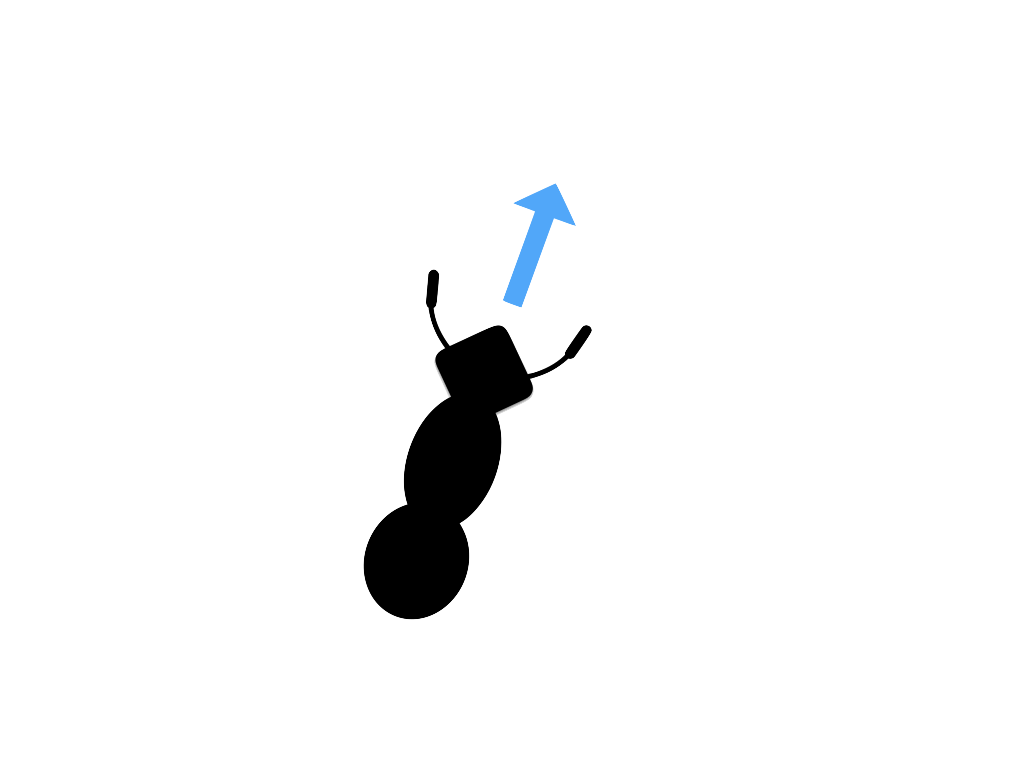
\includegraphics[width=0.20\textwidth]{images/model_components_cartoons_001} &
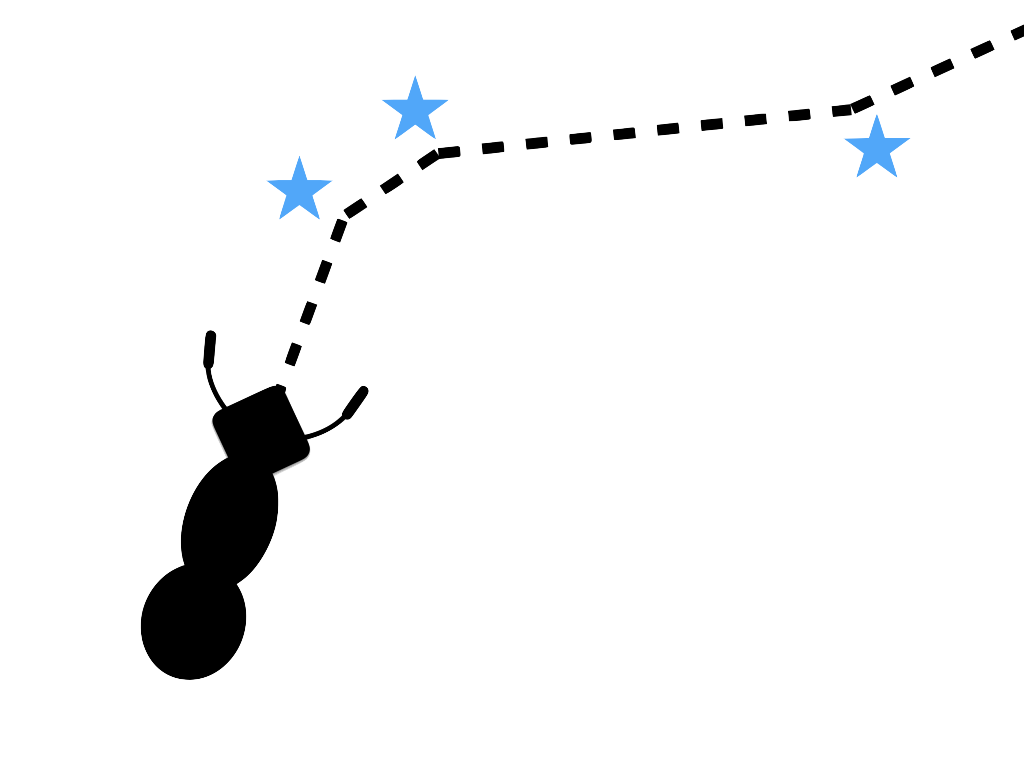
\includegraphics[width=0.20\textwidth]{images/model_components_cartoons_009} &
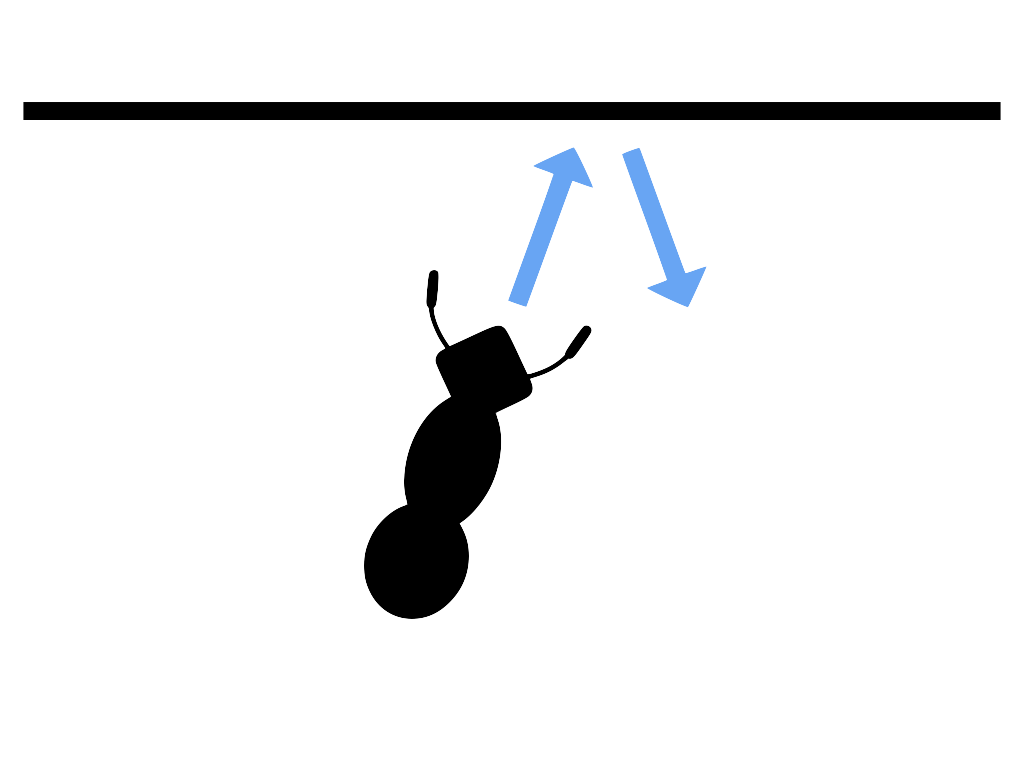
\includegraphics[width=0.20\textwidth]{images/model_components_cartoons_013} \\
\begin{spacing}{1.0}
{\footnotesize
Self Propulsion}
\end{spacing} &
\begin{spacing}{1.0}
{\footnotesize
Random Reorientation}
\end{spacing} &
\begin{spacing}{1.0}
{\footnotesize
Containment}
\end{spacing} 
\\[-0.75cm]
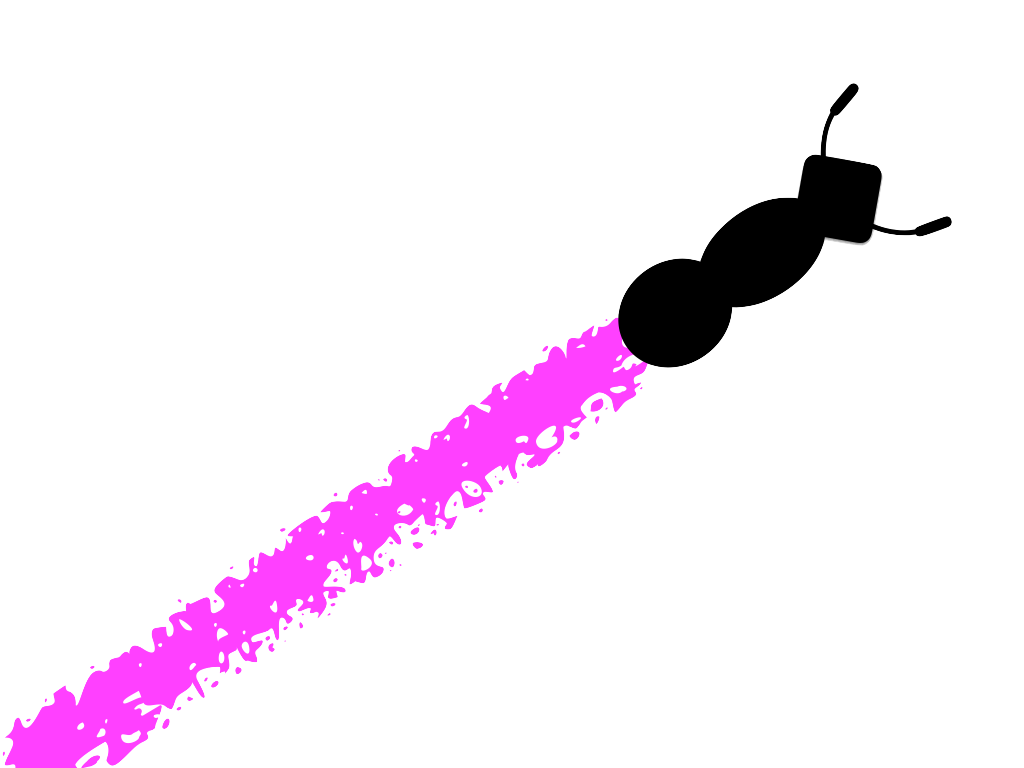
\includegraphics[width=0.20\textwidth]{images/model_components_cartoons_006} &
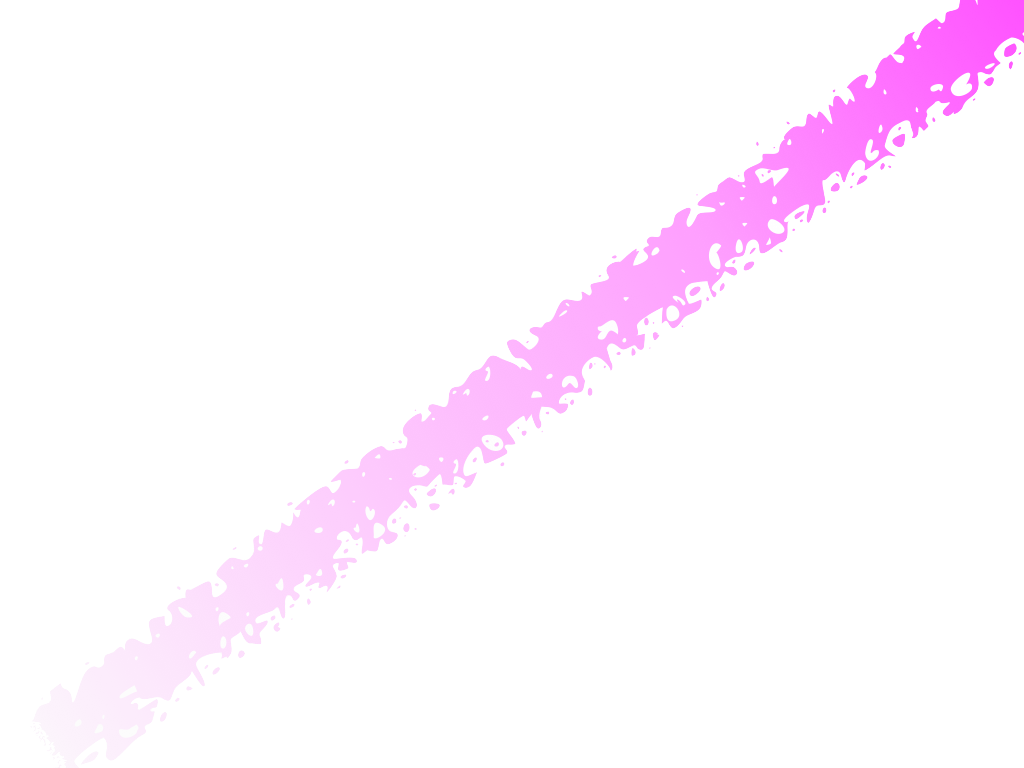
\includegraphics[width=0.20\textwidth]{images/model_components_cartoons_008} &
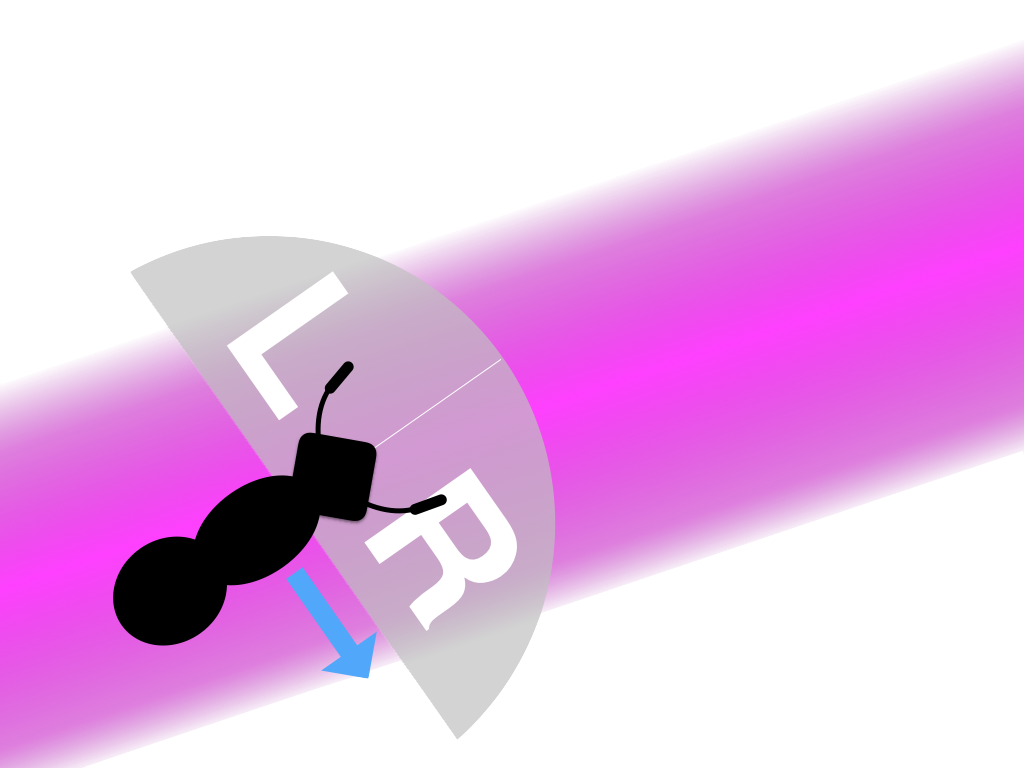
\includegraphics[width=0.20\textwidth]{images/model_components_cartoons_007} \\
\begin{spacing}{1.0}
\raggedright{\footnotesize
Pheromone Deposit}
\end{spacing} &
\begin{spacing}{1.0}
{\footnotesize
Pheromone Evaporation}
\end{spacing} &
\begin{spacing}{1.0}
{\footnotesize
Pheromone Response}
\end{spacing} \\[-0.75cm]
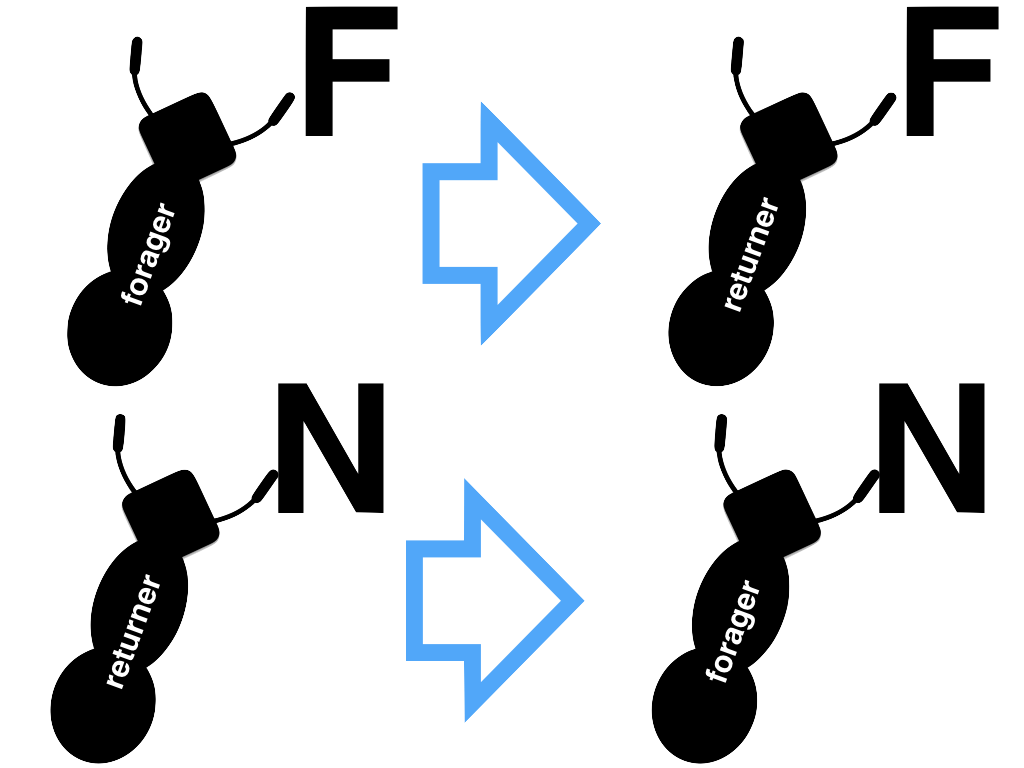
\includegraphics[width=0.20\textwidth]{images/model_components_cartoons_005} &
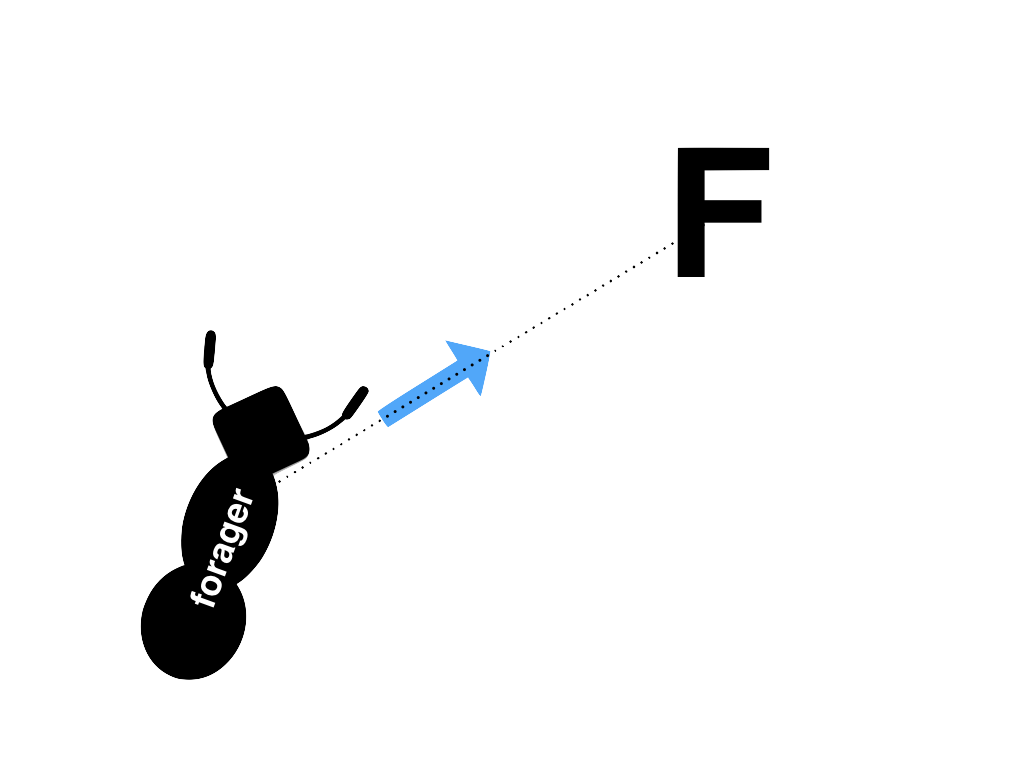
\includegraphics[width=0.20\textwidth]{images/model_components_cartoons_004} &
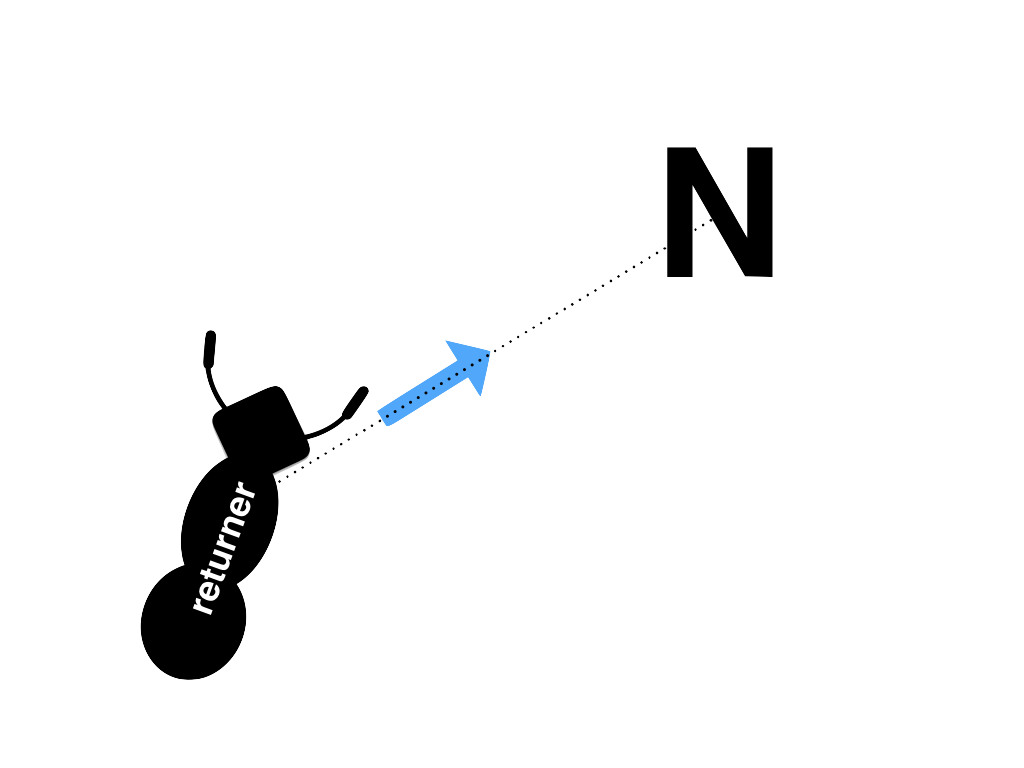
\includegraphics[width=0.20\textwidth]{images/model_components_cartoons_002} \\ 
\begin{spacing}{1.0}
\raggedright{\footnotesize
Forager/Returner Roles}
\end{spacing} &
\begin{spacing}{1.0}
{\footnotesize
Food Attraction}
\end{spacing} &
\begin{spacing}{1.0}
{\footnotesize
Nest Attraction}
\end{spacing} \\[-0.75cm]
\end{tabular}
\caption{Major modeling considerations}
\end{figure}
\end{frame}
\end{subsection}